\section{Affichage des erreurs et warnings}
\noindent Lors de la compilation d'un fichier Prolog, il est possible que des erreurs ou des warnings apparaissent
qui ne sont pas détectés plus tôt car ce ne sont pas des erreurs de syntaxe.
\newdoubleline
Par exemple, il est possible d'avoir une erreur de prédicats non définis ou une erreur de variables non définies ou simplement des avertissements par rapport à des variables "Singletons".

\subsection{L'idée}
\noindent L'idée est de récupérer les erreurs et les warnings de la compilation du fichier Prolog et de les afficher dans l'éditeur Prolog.
\newdoubleline
Ceci implique différentes contraintes:
\begin{enumerate}
    \item Il faut prendre en compte que la compilation doit avoir lieu en temps réel et en arrière plan.
    \item La compilation doit avoir lieu sur macOS, Linux et Windows.
    Ce qui implique de mettre en place un système multi-plateforme.
    \item La compilation doit aussi être dans un thread séparé pour ne pas bloquer l'interface et ne pas ralentir l'éditeur.
\end{enumerate}

\subsection{La mise en pratique}
\noindent Pour la compilation, nous utiliserons le SDK relatif au projet ouvert.
\newdoubleline
Pour l'aspect compilation en temps réel, JetBrains propose une classe nommée "ExternalAnnotator" qui permet de faire des annotations externes.
\newdoubleline
Cette classe permet de faire des annotations externes, notamment à l'aide d'un thread séparé. La classe se présente comme suit:
\begin{enumerate}
    \item \textbf{collectInformation}: Cette méthode permet de récupérer les informations afin de générer les annotations.
    C'est dans cette partie que le lancement de la compilation aura lieu.
    \item \textbf{doAnnotate}: Cette méthode permet de générer les annotations pour chaque ligne.
\end{enumerate}

\noindent Voici le code permettant de récupérer un processus de compilation Prolog:
\begin{lstlisting}[label={lst:get_prolog_process}, caption={Méthode de créer un processus de compilation Prolog}, language=java]
    public static Process getProcess(Path compiler, Path filePath) throws IOException, CantRunException {
        Process p;
        BufferedWriter writer;

        if (SystemInfo.isWindows) {
            p = Runtime.getRuntime().exec("cmd.exe /min");
            writer = new BufferedWriter(new java.io.OutputStreamWriter(p.getOutputStream()));
            writer.write("set LINEDIT=gui=no"); //Prevent windows from opening a console
            writer.newLine();
            writer.write(compiler.toString()); //Launch the compiler
            writer.newLine();
            writer.flush(); //Flush the stream
        } else {
            p = Runtime.getRuntime().exec(compiler.toString());
            writer = new BufferedWriter(new java.io.OutputStreamWriter(p.getOutputStream()));
        }

        writer = new BufferedWriter(new java.io.OutputStreamWriter(p.getOutputStream()));
        String normalizedFilePath = filePath.toString().replace("\\", "/"); //Mandatory for windows
        String goal = "consult('" + normalizedFilePath + "').";
        writer.write(goal);
        writer.newLine();
        writer.flush();
        writer.close();
        return p;
    }
\end{lstlisting}

\noindent Au final, voici le résultat en action dans l'éditeur :
\begin{figure}[h]
    \centering
    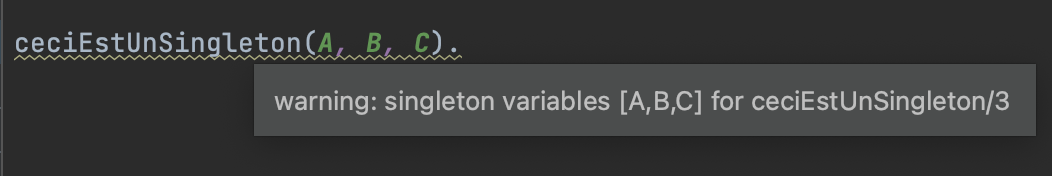
\includegraphics[width=0.8\textwidth]{images/background_compilation.png}
    \caption{Affichage d'avertissement grâce à la compilation}
    \label{fig:compilation_warnings}
\end{figure}